
\section{Spell checker}
\index{secrets!spell checker}

\textit{\htmladdnormallink{See the steps to be followed in order to install a dictionary}{\#configuration\_spellerinstalation}}.
After installing the dictionary, Tinn-R will automatically load it upon starting a new session.
To perform a spell check press \texttt{CTRL + F8} to open the tools window, and then click on Spell.
Go to the editor task bar where it says \texttt{ABC}.
The arrow to the left allows you to choose the language in which the text is written.
Click on \texttt{ABC}. All corrections are automatically added to the text. After finishing this process,
focus again on the editor and press \texttt{CTRL + S} to save all corrections.

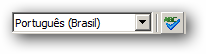
\includegraphics[scale=0.50]{./res/secrets_spell.png}
